\documentclass[11pt]{scrartcl}
\usepackage{polski}
\usepackage[polish]{babel}

\usepackage{graphicx, float, caption, subcaption}
\usepackage{amsmath}
\usepackage{tabularx}
\usepackage{multirow}
\graphicspath{{images/}}

\title{Laboratorium 3 - Triangulacja wielokątów monotonicznych}
\author{Mateusz Podmokły - II rok Informatyka WI}
\date{15 listopad 2023}

\begin{document}
    \maketitle
    \section{Specyfikacja użytego środowiska}
    Specyfikacja:

    \begin{itemize}
        \item Środowisko: Jupyter Notebook,
        \item Język programowania: Python,
        \item System operacyjny: Microsoft Windows 11,
        \item Architektura systemu: x64.
    \end{itemize}

    \section{Przebieg ćwiczenia}
    Ćwiczenie polega na zaimplementowaniu algorytmu sprawdzania, czy podany wielokąt
    jest wielokątem y-monotonicznym oraz algorytmu triangulacji takich wielokątów.
    Dodatkowo napisane zostało narzędzie pozwalające zadawać wielokąty przy użyciu
    myszki.

    \subsection{Sprawdzanie y-monotoniczności}
    Y-monotoniczność została sprawdzona poprzez analizę kolejnych wierzchołków. Jeżeli
    więcej niż jeden raz odwrócona była monotoniczność współrzędnej $y$ wierzchołków,
    znaczyło to, że wielokąt nie jest y-monotoniczny.

    \begin{figure}[H]
        \centering
        \begin{minipage}{0.45\linewidth}
          \centering
          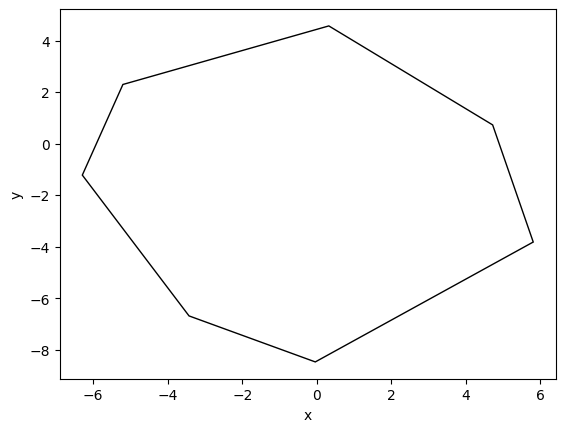
\includegraphics[width=1\linewidth]{3_1.png}
          \caption{Wielokąt y-monotoniczny.}
        \end{minipage}
        \begin{minipage}{0.45\linewidth}
          \centering
          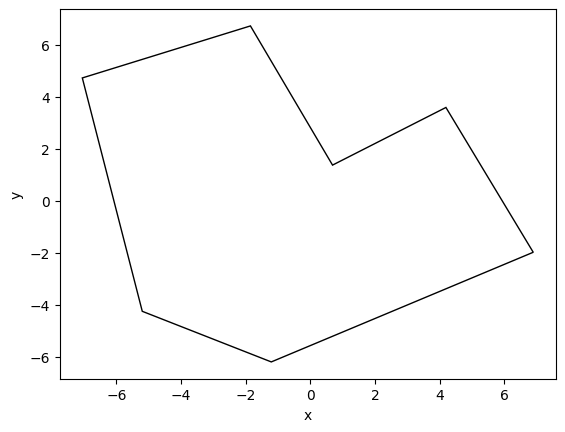
\includegraphics[width=1\linewidth]{3_2.png}
          \caption{Nie jest y-monotoniczny.}
        \end{minipage}
    \end{figure}

    \subsection{Klasyfikacja wierzchołków wielokąta}
    Wierzchołki wielokąta zostały podzielone na 5 kategorii:    

    \begin{itemize}
        \item początkowe, gdy obaj sąsiedzi leżą poniżej i kąt wewnętrzny ma mniej
        niż 180 stopni
        \item końcowe, gdy obaj sąsiedzi leżą powyżej i kąt wewnętrzny ma mniej
        niż 180 stopni
        \item dzielący, gdy obaj sąsiedzi leżą poniżej i kąt wewnęntrzny ma więcej
        niż 180 stopni
        \item łączący, gdy obaj sąsiedzi leżą powyżej i kąt wewnęntrzny ma więcej
        niż 180 stopni
        \item prawidłowe, pozostałe przypadki, jeden sąsiad powyżej, drugi poniżej
    \end{itemize}

    \begin{figure}[H]
        \centering
        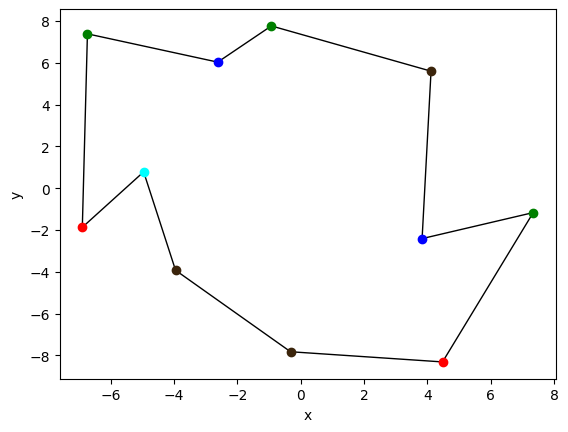
\includegraphics[width=0.8\linewidth]{3_3.png}
        \caption{Wielokąt z pokolorowanymi wierzchołkami.}
    \end{figure}

    \subsection{Triangulacja wielokąta}

    Wielokąt został podzielony na dwa łańcuchy wierzchołków - lewy i prawy. Następnie
    oba łańcuchy zostały połączone w jeden, co dało ciąg wierzchołków posortowanych
    według współrzędnej $y$ w czasie $O(n)$, gdzie $n$ to liczba wierzchołków. W celu
    znajdowania sąsiadów danego wierzchołka utworzona została tablica oryginalnej
    kolejności wierzchołków w wielokącie (w progranie nazwana $order$). Triangulacja
    jest przechowywana w postaci listy par indeksów wierzchołków między którymi
    występują połączenia tworzące triangulację. Wybrane struktury przechowujące
    wielokąt oraz triangulację pozwoliły na uzyskanie złożoności obliczeniowej
    całości algorytmu $O(n)$.

    \begin{figure}[H]
        \centering
        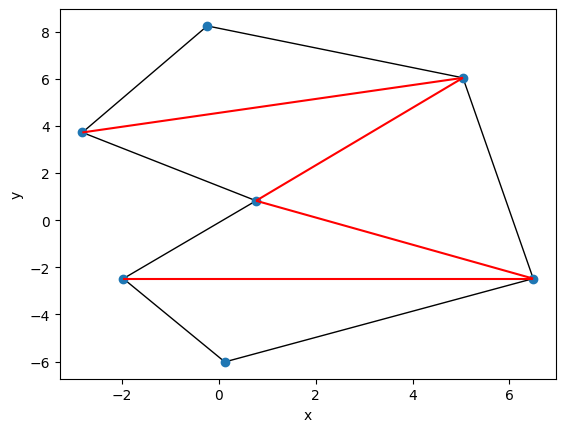
\includegraphics[width=0.8\linewidth]{3_4.png}
        \caption{Przykładowa triangulacja.}
    \end{figure}

    \section{Analiza otrzymanych triangulacji}
    \subsection{Wielokąty użyte do testów}

    \begin{figure}[H]
        \centering
        \begin{minipage}{0.45\linewidth}
          \centering
          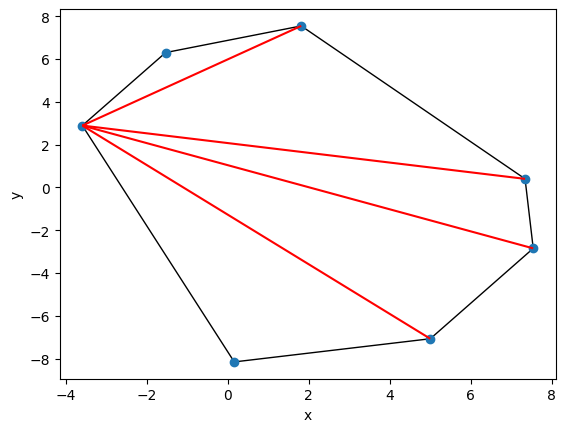
\includegraphics[width=1\linewidth]{3_5.png}
          \caption{}
        \end{minipage}
        \begin{minipage}{0.45\linewidth}
          \centering
          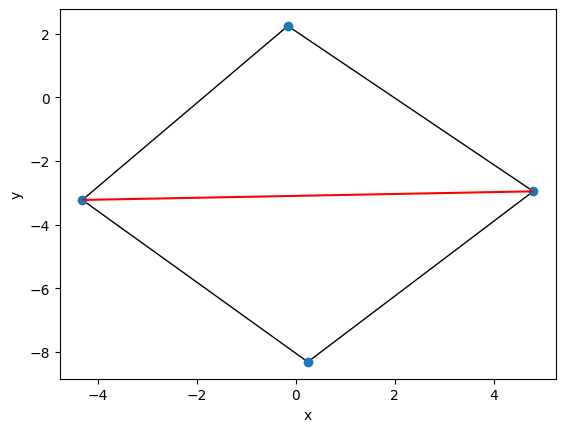
\includegraphics[width=1\linewidth]{3_6.png}
          \caption{}
        \end{minipage}
    \end{figure}

    \begin{figure}[H]
        \centering
        \begin{minipage}{0.45\linewidth}
          \centering
          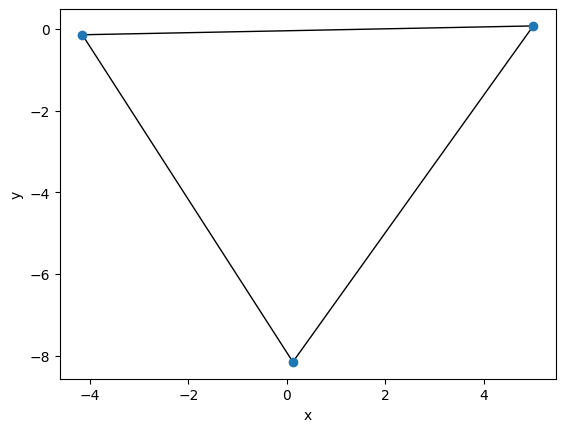
\includegraphics[width=1\linewidth]{3_7.png}
          \caption{}
        \end{minipage}
        \begin{minipage}{0.45\linewidth}
          \centering
          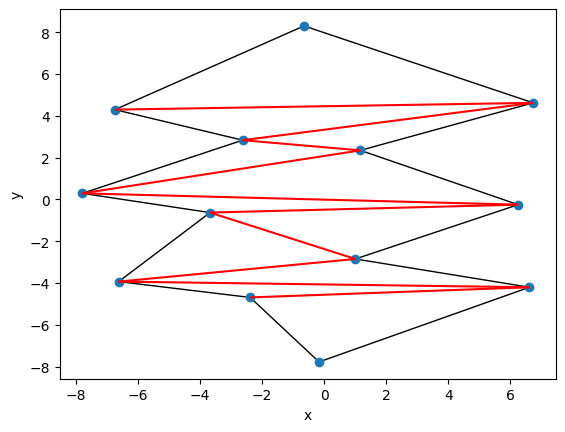
\includegraphics[width=1\linewidth]{3_8.png}
          \caption{}
        \end{minipage}
    \end{figure}

    \begin{figure}[H]
        \centering
        \begin{minipage}{0.45\linewidth}
          \centering
          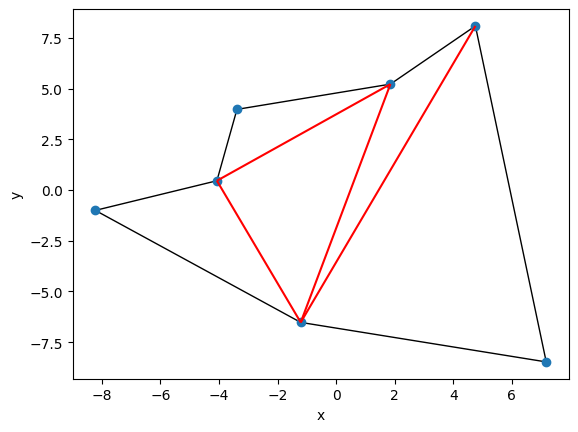
\includegraphics[width=1\linewidth]{3_9.png}
          \caption{}
        \end{minipage}
        \begin{minipage}{0.45\linewidth}
          \centering
          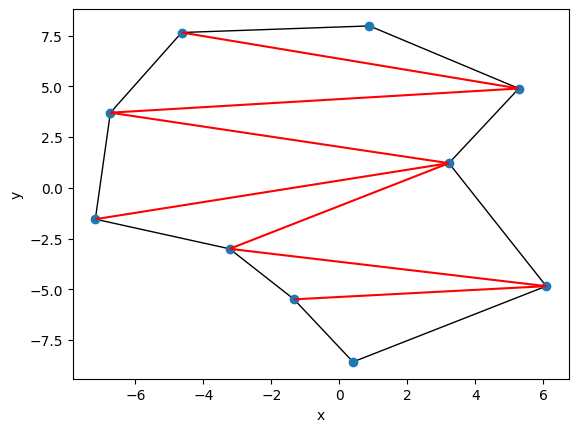
\includegraphics[width=1\linewidth]{3_10.png}
          \caption{}
        \end{minipage}
    \end{figure}

    \subsection{Analiza wyników}
    Pierwszy wielokąt (rys. 5) posiada wszystkie punkty lewego łańcucha powyżej
    prawego, dlatego najniższy punkt lewego łańcucha jest połączony ze wszystkimi
    z prawego. W drugim (rys. 6) znajduje się tylko jeden odcinek podziałowy, ze względu na
    to, że ma tylko 4 boki. Trzeci wielokąt (rys. 7) jest trójkątem, więc nie wymaga
    żadnych podziałów. W następnym (rys. 8) kolejne wierzchołki pojawiają się naprzemiennie
    w łańcuchu prawym oraz lewym, dlatego podziały przechodzą po kolei od góry do dołu.
    Rysunek 9 zawiera wielokąt z wklęsłościami, który wymaga "odcięcia" wklęsłości.
    Ostatni (rys. 10) to połączenie naprzemiennych podziałów z wielokrotnymi podziałami
    do niższych wierzchołków.

    \section{Wnioski}
    Użyte wielokąty pozwoliły przetestować algorytm triangulacji na różnych rodzajach
    wielokątów, dając odmienne efekty podziałów na trójkąty. Warto zaznaczyć, że wszystkie
    były y-monotoniczne. Zastosowany algorytm jest wydajny bez względu na rodzaj
    triangulowanego wielokąta, ponieważ posiada złożoność obliczeniową $O(n)$. Jednak
    nadaje się on jedynie do wielokątów y-monotonicznych, co może być sporym ograniczeniem.

\end{document}
